
% JuliaCon proceedings template
\documentclass{juliacon}
\setcounter{page}{1}
\usepackage{amsmath,booktabs,mathtools,amssymb}
\newcommand{\term}[1]{\emph{#1}}
\newcommand{\e}{\ensuremath{\mathrm{e}}}
\newcommand{\im}{\ensuremath{\mathrm{i}}}
\newcommand{\LieGroupsVersion}{0.1.6}
%
\hypersetup{colorlinks=true}
%
\begin{document}

% **************GENERATED FILE, DO NOT EDIT**************

\title{My JuliaCon proceeding}

\author[1]{1st author}
\author[1, 2]{2nd author}
\author[2]{3rd author}
\affil[1]{University}
\affil[2]{National Lab}

\keywords{Julia, Optimization, Game theory, Compiler}

\hypersetup{
pdftitle = {My JuliaCon proceeding},
pdfsubject = {JuliaCon 2022 Proceedings},
pdfauthor = {1st author, 2nd author, 3rd author},
pdfkeywords = {Julia, Optimization, Game theory, Compiler},
}


% TODO : How to specify an email-address?
\maketitle

\begin{abstract}
    \href{https://juliamanifolds.github.io/LieGroups.jl/stable/}{\texttt{LieGroups.jl}} is a
    Julia package that provides an interface to define Lie groups as well as the corresponding Lie algebra and Lie group actions. The package also offers a well-documented, performant, and well-tested library of existing Lie groups, their algebra and corresponding group actions.

    This paper presents the main features of the interfaces and how that is integrated within
    the \verb|JuliaManifolds| ecosystem. We further present an overview on existing Lie groups
    implemented in \verb|LieGroups.jl| as well as how to get started to use the package in practice.
\end{abstract}
%
\section{Introduction}%
\label{sec:Introduction}
%
In many situations, one encounters data that does not reside in a vector space.
We can hence not use standard linear algebra tools to work with such data.
For example in robotics, the configuration space of a rigid body in three-dimensional
space is given by the special Euclidean group \(\mathrm{SE}(3)\),
consisting of all translations and rotations.
A subset of these is the space of rotations, given by the special orthogonal group \(\mathrm{SO}(3)\),
or more generally \(\mathrm{SO}(n)\) in \(n\)-dimensional space.

These spaces are examples of Lie groups, formally defined as a smooth manifold equipped with a group structure.
They have applications in physics, robotics, stochastic processes, information geometry, and many other areas see~\cite{Chirikjian:2009,Chirikjian:2012},
but are also interesting from their mathematical viewpoint~\cite{HilgertNeeb:2012}
and their numerical aspects, for example when solving differential equations on Lie groups~\cite{Munthe-Kaas:1998}.

The package~\href{https://juliamanifolds.github.io/LieGroups.jl/stable/}{\texttt{LieGroups.jl}}\footnote{%
Available at~\href{https://juliamanifolds.github.io/LieGroups.jl/stable/}{juliamanifolds.github.io/LieGroups.jl/stable/},
see also the zenodo archive~\cite{LieGroups.jl}.%
}
provides an easy access to both defining and using Lie groups within
the Julia programming language~\cite{bezanson2017julia} by defining an interface of Lie groups, as well as implementing a library of Lie groups, that can directly be used.

This paper provides an overview of the main features of \verb|LieGroups.jl| as of version \LieGroupsVersion{}.
After introducing the necessary mathematical background and notation in Section~\ref{sec:Notation},
we present the interface in Section~\ref{sec:Interface}, split into the Lie group, the Lie algebra, and group actions.
In Section~\ref{sec:LieGroups}, we present an overview of currently implemented Lie groups.
Finally, in Section~\ref{sec:Example}, we demonstrate how to get started and use \verb|LieGroups.jl|.

\section{Mathematical Background}%
\label{sec:Notation}

\begin{figure}
    \centering
    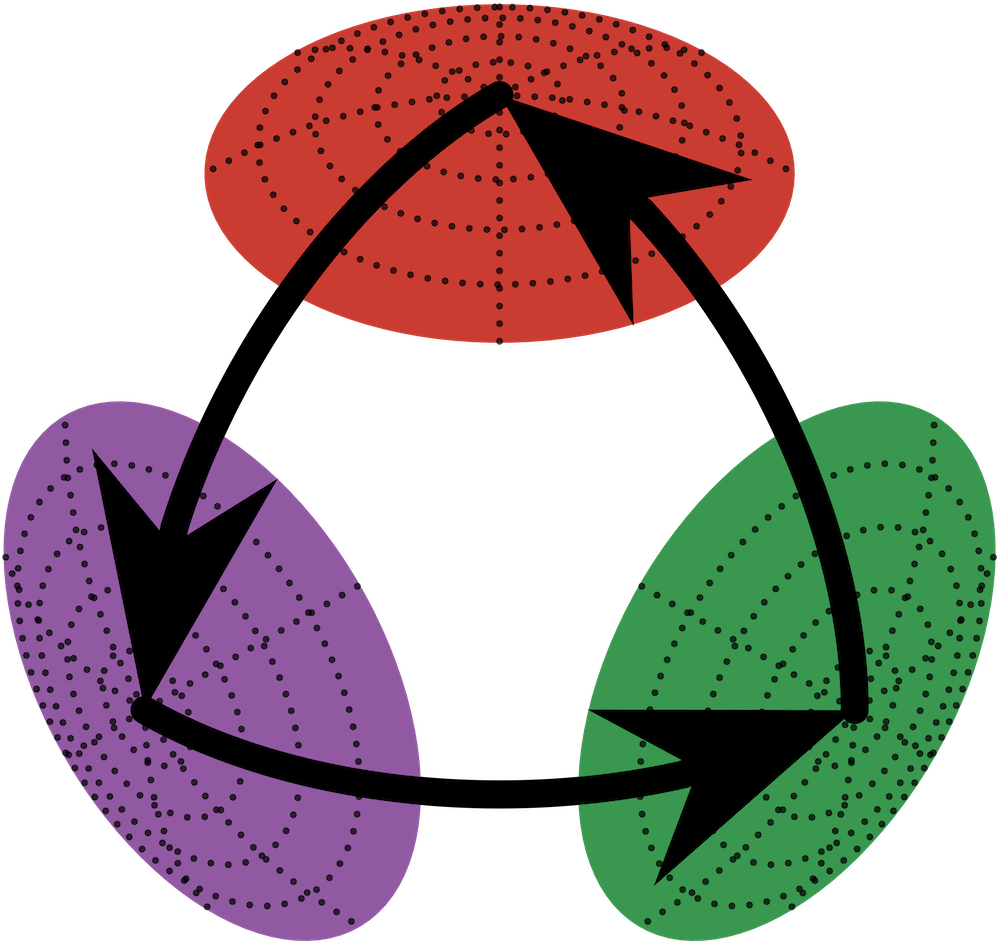
\includegraphics[width=0.12\textwidth]{logo.png}
    \vspace{.5\baselineskip}
    \caption*{Logo of \texttt{LieGroups.jl}.}%
    \label{fig:liegroups_logo}
\end{figure}

The following notation and definitions follow the text book~\cite{HilgertNeeb:2012},
for more details on Riemannian manifolds, see also~\cite{DoCarmo:1992}.

\subsection{Lie groups}
We denote a Lie group by \(\mathcal{G} = (\mathcal{M}, \cdot)\) where \(\mathcal{M}\) is a smooth manifold and \(\cdot\) is the group operation.
A smooth manifold \(\mathcal{M}\) is a topological space that is locally isomorphic to an Euclidean space \(\mathbb{R}^n\) for some \(n \in \mathbb{N}\), but globally may have a different topology.
We call \(n\) the dimension of the manifold \(\mathcal{M}\), denoted by \(\dim(\mathcal{M}) = n\).
As an example, take the \(2\)-dimensional sphere
\begin{equation*}
\mathbb{S}^2 = \bigl\{ p \in \mathbb{R}^3 \bigm| \lVert p\rVert = 1\bigr\},
\end{equation*}
% MB: maybe it would be better to replace it with an example that can have a group structure? For example the 3-dimensional sphere?

which locally looks like \(\mathbb{R}^2\), think of charts in an atlas, but globally it is not.
Finally we denote the tangent space at a point \(p \in \mathcal{M}\) by \(T_p\mathcal{M}\). This can be thought of as all “velocities” (direction and speed) in which a curve can “pass through” a point. Formally it is set the equivalence classes of derivatives of smooth curves. Each tangent space $T_p\mathcal M$ is a $n$-dimensional vector space and we call the disjoint union of all tangent spaces
\begin{equation*}
    T\mathcal M = \dot\bigcup_{p \in \mathcal M} T_p\mathcal M
\end{equation*}
the \term{tangent bundle} of $\mathcal M$.
\\
As a group operation \(\cdot\colon\mathcal{G} \times \mathcal{G} \to \mathcal{G}\) has to satisfy the group axioms: associativity, existence of an identity element \(e \in \mathcal{G}\), and existence of inverses \(g^{-1} \in \mathcal{G}\) for all \(g \in \mathcal{G}\). Furthermore the group operation \(\cdot\) (on \( \mathcal{G}\times\mathcal{G} \)) and the inversion map \(\iota\colon\mathcal{G} \to \mathcal{G}, g \mapsto g^{-1}\) have to be smooth maps.
As an example, consider the special orthogonal group \(\mathrm{SO}(n)\), consisting of all \(n \times n\) orthogonal matrices, with determinant \(1\), that is for \(p\in \mathrm{SO}(n)\), we have \(p^{\mathrm{T}} p = I\) and \(\det(p) = 1\) together with the group operation \(\cdot\) given by matrix multiplication.
For $n=2$ these are rotations in the plane, hence each operation can be identified with an angle $\alpha \in [-\pi, \pi)$\footnote{Note that the identification is not continuous.}, or, continuously, with the circle. % chktex 9ok
The identity element is given by the identity matrix \(I\) (or the angle $\alpha=0$) and the inverse of a rotation matrix is given by its transpose (or an angle $-\alpha$). % -(-\pi) would be out of the range

\subsection{Tangent spaces and the Lie algebra} The tangent space at the identity element \(e \in \mathcal{G}\), denoted by \(\mathfrak{g} = T_e\mathcal{G}\), plays a special role and is called the \term{Lie algebra} of the Lie group \(\mathcal{G}\).
The reason is that to represent arbitrary tangent vectors $X \in T_g\mathcal{G}$ at a point $g \in \mathcal{G}$ we can use the group operation: we denote by $\lambda_g(h) = g \cdot h$ the left multiplication with $g, h \in \mathcal{G}$.
Then, using the differential (or push forward) $D\lambda_g(h)\colon T_h\mathcal G \to T_{g\cdot h}\mathcal G$\footnote{\color{red} MB: TODO: does the reader know that a differential is? (RB) Sure I can expand on that, I wrote a sentence more further below to get from differential to Jacobian, so I can also add a sentence there as well.}, we can generate a so-called \term{left-invariant vector field} $\mathcal X(g) \coloneqq D\lambda_g(e)[X]$ which is uniquely determined by the choice of $X \in \mathfrak{g}$.%
\footnote{Analogously, one can use the right multiplication $\rho_g(h) = h \cdot g$ and its differential $D\rho_g(h)$ to define right-invariant vector fields. \texttt{LieGroups.jl} uses left-invariant vector fields as default.}%
Hence we can identify tangent vectors $\mathcal X(g) \in T_g\mathcal G$ at arbitrary points $g \in \mathcal G$ with $X$ from the Lie algebra $\mathfrak{g}$.
\\
As a first example, consider $\mathcal G = (\mathbb R^n, +)$, where the tangent space at any point $g$ is again $\mathbb R^n$, especially at the identity $e=0$. We further have $\lambda_g(h) = g + h$ and hence $D\lambda_g(h)[X] = X$ for all $g, h, X \in \mathbb R^n$.
Here, a tangent vector $X$ induces the constraint vector field $\mathcal X(g) = X$ for all $g \in \mathbb R^n$.\\
As a second example, consider again the special orthogonal group $\mathrm{SO}(n)$.
The tangent space at the identity element $e = I$ is given by the Lie algebra $\mathfrak{so}(n) = T_e\mathrm{SO}(n) = \{ X \in \mathbb{R}^{n \times n} \mid X = -X^{\mathrm{T}} \}$ consists of all skew-symmetric $n \times n$ matrices.
For $g, h \in \mathrm{SO}(n)$ and $X \in \mathfrak{so}(n)$ we have $\lambda_g(h) = g \cdot h$ and hence $D\lambda_g(h)[X] = g \cdot X$. Here, the tangent vector $X \in \mathfrak{so}(n)$ induces the left-invariant vector field $\mathcal X(g) = g \cdot X \in T_g\mathrm{SO}(n)$, $g \in \mathrm{SO}(n)$.
In other words, this formulation allows to represent tangent vectors $Y\in T_g\mathrm{SO}(n)$ also using $X = g^{-1}Y \in \frak{g}$.

An important tool to “move around” on the Lie group is the exponential map.
The (Lie group) exponential function \(\exp\colon \mathfrak{g} \to \mathcal{G}\) maps elements from the Lie algebra to the Lie group, and is formally defined \cite[Def.~9.2.2]{HilgertNeeb:2012} by evaluating the unique curve \(\gamma\colon \mathbb{R} \to \mathcal{G}\) that fulfils the differential equation
\begin{equation*}
\gamma'(t) = D\lambda_{\gamma(t)}(e)[X]
\quad\text{ with }\quad\gamma(0) = e \text{ and }\gamma'(0) = X
\end{equation*}
at time $t=1$, that is \(\exp(X) = \gamma(1)\).
This can be interpreted as starting at the identity element \(e \in \mathcal{G}\) and following the curve whose velocity at each point is given by the left-invariant vector field induced by \(X \in \mathfrak{g}\) for one time unit.

For \((\mathbb{R}^n, +)\) the exponential map is given by \(\exp(X) = X\), $X\in \mathbb R^n$ and for \(\mathrm{SO}(n)\) it is given by the matrix exponential \(\exp(X) = \e^{X}\) for all \(X \in \mathfrak{so}(n)\).
Additionally for the unit circle in the complex plane, using the group operation of multiplication, the exponential map is given by the complex exponential \(\exp(X) = \e^{\im X}\) for all \(X \in \mathbb{R}\).

Concerning a metric on the tangent spaces, manifolds are turned into Riemannian manifolds when they are equipped with a Riemannian metric \(\langle \cdot, \cdot \rangle_p\colon T_p\mathcal{M} \times T_p\mathcal{M} \to \mathbb{R}\) for each point \(p \in \mathcal{M}\) that smoothly varies with \(p\).
For Lie groups, we can use a single inner product \(\langle \cdot, \cdot \rangle\) on the Lie algebra \(\mathfrak{g}\) and use the change in representation as mentioned above to define
\begin{equation*}
\langle X, Y \rangle_g = \langle D\lambda_{g^{-1}}(g)[X], D\lambda_{g^{-1}}(g)[Y] \rangle_e
\end{equation*}
for all \(X, Y \in T_g\mathcal{G}\) and \(g \in \mathcal{G}\). Representing tangent vectors at arbitrary points \(g \in \mathcal{G}\) using the Lie algebra \(\mathfrak{g}\) yields here, that we can use the single inner product directly to evaluate this Riemannian metric. Hence representing tangent vectors using the Lie algebra is the default in the following.
\\
For the two examples above we obtain the Euclidean inner product \(\langle X, Y \rangle = X^{\mathrm{T}} Y\) for \(X, Y \in \mathbb{R}^n\) for \((\mathbb{R}^n, +)\) and the Frobenius inner product \(\langle X, Y \rangle = \mathrm{trace}(X^{\mathrm{T}} Y)\), \(X, Y \in \mathfrak{so}(n)\) can be used for \(\mathrm{SO}(n)\).

Note that a Riemannian metric can also be used to define an exponential map using the Levi-Civita affine connection.
This exponential map often differs from the Lie group exponential, in particular many Lie groups, such as the special Euclidean group in two or more dimensions, can not have a metric compatible with the Lie group exponential.

\subsection{Group Actions} A \term{group action} of a Lie group \(\mathcal{G}\) on a smooth manifold \(\mathcal{M}\) is a smooth map \(\sigma\colon \mathcal{G} \times \mathcal{M} \to \mathcal{M}\) such that for all \(g, h \in \mathcal{G}\) and \(p \in \mathcal{M}\) it holds that \(\sigma(e, p) = p\) and \(\sigma(g, \sigma(h, p)) = \sigma(g \cdot h, p)\).\footnote{This is the convention for left actions. Alternatively, right actions fulfil \(\sigma(g, \sigma(h, p)) = \sigma(h \cdot g, p)\).}
Informally a group action describes how elements of the Lie group \(\mathcal{G}\) “act on” points on the manifold \(\mathcal{M}\). As an example, think of the special orthogonal group \(\mathrm{SO}(3)\) acting on points on Euclidean space $\mathbb{R}^3$ “moving” them somewhere by rotating them around the origin. We obtain the group action \(\sigma\colon \mathrm{SO}(3) \times \mathbb{R}^3 \to \mathbb{R}^3\), \(\sigma(R, x) \coloneqq Rx\).

The same action can also be applied to points from the sphere \(\mathbb{S}^2\), resulting in a similar group action \(\sigma\colon \mathbb{SO}(3) \times \mathbb{S}^2 \to \mathbb{S}^2\), \(\sigma(R, p) \coloneqq Rp\).

\section{The interface}\label{sec:Interface}

Since a Lie group \(\mathcal{G}\) consists of two main components, the smooth manifold \(\mathcal{M}\) and the group operation \(\cdot\), we can reuse existing functionality from the existing interface for manifolds provided by \verb|ManifoldsBase.jl|, and later concrete manifolds provided by \verb|Manifolds.jl|~\cite{AxenBaranBergmannRzecki:2023}.
This is done in a transparent way, i.e.\ the \verb|AbstractLieGroup| itself is a subtype of \verb|AbstractManifold| from \verb|ManifoldsBase.jl| and can hence also be used in all existing places, as for example optimization on manifolds provided by \verb|Manopt.jl|~\cite{Bergmann:2022}.
In notation, we use typewriter font to denote functions in the interface, but we keep the same letters of notation as before, i.e.\ $\mathcal G$ for a Lie group is \verb|G| in code, a point $g \in \mathcal G$ is \verb|g| in code, and so on, just that for the Lie algebra we use $\mathfrak g$ in both text and code.

The interface follows the philosophy of \verb|ManifoldsBase.jl|, that the Lie group or algebra is the first argument and even a mutated argument comes second.
Similarly, if a function computes something like a new point on the Lie group or a tangent vector, there also exists a variant, that computes this in-place.
For example \verb|identity_element(G)| returns the identity element $e$ of a Lie group $G$ in a default representation, \verb|identity_element!(G, e)| writes the result into the pre-allocated variable \verb|e|, which can also be used with other representation types.

\subsection{Lie groups}

The main type for Lie Groups is the \verb|LieGroup{|$\mathbb {F}$\verb|, O, M} <: AbstractLieGroup|, which contains a manifold \verb|M <: AbstractManifold{|$\mathbb F$\verb|}| as well as the group operation \verb| O <: AbstractGroupOperation|, where $\mathbb {F}$ is the set of scalars used in the representation of the manifold, usually \(\mathbb {F} = \mathbb{R}\) and in some cases \(\mathbb {F}\) is the field of complex numbers \(\mathbb{C}\) or the ring of quaternions \(\mathbb H\).

In general, when a function within the interfaces of \verb|JuliaManifolds| returns a point, a tangent vector or any other mutable object, there always exist two variants of the function, one that allocates a new object and returns it, and one that takes an additional argument to write the result into. For example for a function \verb|f(G, g)| that returns a point on the Lie group \verb|G|, there also exists a variant \verb|f!(G, h, g)| that computes the result in-place of \verb|h|, possibly using the memory also for interims results. By default the allocating variant is implemented by allocating memory accordingly and calling the in-place variant. This default can be overriden, for example for performance reasons.

\subsubsection*{Topological functions}
Points and tangent vectors can be represented by the same Julia objects, although they are distinct from a topological viewpoint.%
\footnote{\texttt{LieGroups.jl} introduces a \texttt{AbstractLieGroupPoint <: AbstractManifoldPoint}, that is used to represent points on the Lie group.
This abstract supertype is not necessary, points can be represented by arrays or other types as well.}
Separate types are necessary when one Lie group has \emph{different representations} of points, that have to be distinguished. When there are different representations, it is recommended to introduce a point type for each representation and make the default one fall back to (just) using arrays.
Several functions in the interface return points or tangent vectors, where the type might not be known from the input argument. For such a function, for example again a function \verb|f(G)| a positional argument \verb|T| can be used to specify the desired return type, i.e.\ \verb|f(G, T)| returns a point or tangent vector of type \verb|T|.
The in-place variant does not require this, since in its signatgure of the form \verb|f!(G, g::T)| the type \verb|T| is known from the argument \verb|g|.

Alternatively to points, also different manifolds can be used. This is for example the case for the circle group \(\mathbb{S}^1\), which can be represented as angles, points on the unit circle in \(\mathbb{R}^2\) or as complex numbers with unit norm, all three of which are different manifolds to be used internally. To access the underlying manifold, the function \verb|base_manifold(G)| is provided.



The following functions are available and pass directly to the underlying manifold interface from \verb|ManifoldsBase.jl|:
\verb|is_approx(G, g, h)| to check for (approximate) equality of two points,
\verb|is_point(G, g; error=:none)| to check if a point is a valid point on the manifold, where the keyword can be used to throw an \verb|:error|, a \verb|:warn| or an \verb|:info|.
Similarly
\verb|manifold_dimension(G)| to get the dimension of the manifold,
\verb|project(G, q)|%
%\footnote{in-place variant \texttt{project!(G, p, q)}.} to project a point onto the manifold, as well as
\verb|rand(G)| and \verb|rand(rng, G)|%
%\footnote{in-place variant \texttt{rand!(G, p)} and \texttt{rand!(rng, G, p)}, respectively.}
to sample a random point from the manifold using a random number generator \verb|rng| also pass directly on to the manifold.
To access the underlying manifold of the Lie group one can use \verb|base_manifold(G)|.


\subsubsection*{Group operation related functions}

\begin{table}
    \centering
    \caption{Group operations available in \texttt{LieGroups.jl}.}
    \begin{tabular}{@{}ll@{}}
        \toprule
        \textbf{Group operation} $\cdot$ & comment/code\\
        \midrule
        \verb|AdditionGroupOperation| & falls back to \verb|+|\\
        \verb|AbelianMultiplicationGroupOperation| & falls back to \verb|*|\\
        \verb|LeftMatrixMultiplicationGroupOperation| & falls back to \verb|*|\\
        \verb|PowerGroupOperation{Op}| & \verb|PowerLieGroup|\\
        \verb|ProductGroupOperation{Ops}| & product Lie groups\\
        \verb|SemidirectProductGroupOperation| & semidirect products\\
        \bottomrule
    \end{tabular}
    \label{tab:GroupOperations}
\end{table}

For the group operation \(\cdot\) of a Lie group \(\mathcal{G}\), the abstract supertype \verb|AbstractGroupOperation| is mandatory. There are two main group operation types provided in \verb|LieGroups.jl|. On the one hand operations that fall back to using $\cdot = +$ or $\cdot = *$, where the latter has two variants, the one where it is Abelian (like for numbers) and where it is not (like for matrices).
On the other hand, specific meta groups like the (direct) product of two or more groups, the case where the product is taken for just one group, i.e.\ the power group, or semidirect products. The available group operation types are summarized in Table~\ref{tab:GroupOperations}. More on these meta groups is explained in Subsection~\ref{subsec:MetaLieGroups}.

For all these group operations, the following functions have default implementations. They might not be the most performant ones for every case, but provide working implementations out-of-the-box.
It is always possible to override these by defining a new group operation type and implementing the following functions for a \verb|LieGroup| with that new group operation type.

To avoid unnecessary allocations, the identity element can be used without allocations, calling \verb|e = IdentityElement(G)| or \verb|IdentityElement(op)| where \verb|op| is the group operation of \verb|G|. If the actual value is needed, one can call

\verb|identity_element(G)| or \verb|identity_element(G, typeof(g))|, where \verb|g| is an element of the group. The first variant will always generate a point in the default representation of the group, while the latter will generate a point in the same representation as \verb|g|.%
\footnote{The in-place variant \texttt{identity\_element!(G, e::T)} infers the representation from the type \texttt{T} of \texttt{e}.}

The two central functions are \verb|compose(G, g, h)|
%\footnote{in-place variant \texttt{compose!(G, k, g, h)}.}
to compute the group operation \(g \cdot h\) for two points \(g, h \in \mathcal{G}\) and the inverse \verb|inv(G, g)|
%\footnote{in-place variant \texttt{inv!(G, h, g)}.}
which computes \(g^{-1}\) for a point \(g \in \mathcal{G}\).

Another function is $c_g(h) = g \cdot h \cdot g^{-1}$ called \term{conjugation}, which is available as \verb|conjugate(G, g, h)|%
%\footnote{in-place variant \texttt{conjugate!(G, k, g, h)}.}
.

For these three functions, also the differentials are available: adding a \verb|diff_| prefix to the function name and a final argument for the Lie algebra tangent vector, for compose additionally the argument with which to  differentiate to, i.e.\ \verb|diff_left_compose(G, g, h, X)| and \verb|diff_right_compose(G, g, h, X)|, respectively%
%\footnote{in-place variants have a second argument \texttt{Y} to compute the result in.}
.

Finally, there is a specific function for the differential of the conjugate at the identity $h=e$ called \verb|adjoint(G, g, X)|
%\footnote{in-place variant \texttt{adjoint!(G, Y, g, X)}.}
as well as the combinations \verb|inv_left_compose(G, g, h)|
%\footnote{in-place variant \texttt{inv\_left\_compose!(G, k, g, h)}}
for computing $g^{-1}\cdot h$ and \verb|inv_right_compose(G, g, h)|
%\footnote{in-place variant \texttt{inv\_right\_compose!(G, k, g, h)}
for computing $g \cdot h^{-1}$. All three fall back to the previously defined functions, but provide an interface to possibly implement more efficient variants in case such exist.

\subsubsection*{Exponential and logarithm.}

In \verb|LieGroups.jl|, the exponential function is given by \verb|exp(G,X)|%
%\footnote{in-place variant \texttt{exp!(G, g, X)}.}
.
If we want to “start walking” from another point, we can “move” (or interpret $X$) as being from the tangent space at some point $g$ and obtain by the chain rule the \term{exponential function} $\exp_g\colon\frak g\to\mathcal G$ defined by $\exp_g(X)\coloneqq g \cdot \exp(X)$.
In \verb|LieGroups.jl|, the exponential map is implemented as \verb|exp(G, g, X)|%
%\footnote{in-place variant \texttt{exp!(G, h, g, X)}.}
.
As a word of carefulness, note that on the underlying manifold, there is a further exponential map, the Riemannian exponential map. The Riemannian exponential map \verb|exp(M, p, X)|
%\footnote{with the same in-place signature as before \texttt{exp!(M, q, p, X)}.}
can be distinguished in that the first argument is a manifold, and the tangent vector \verb|X| has to be from the tangent space at the point \verb|p| on the manifold.
Here, again, to access the Riemannian exponential, one can use the base manifold of the Lie group, i.e.\ \verb|exp(base_manifold(G), g, X)| and have to make sure that \verb|X| is from the tangent space at \verb|g|.

Locally around the identity element $e\in\mathcal G$, the exponential map is a diffeomorphism, i.e.\ there exists an inverse map on some neighbourhood of $e$. The logarithmic function \(\log\colon \mathcal{G} \to \mathfrak{g}\) and logarithmic map \(\log_g\colon \mathcal{G} \to \mathfrak{g}\)have the function signatures \verb|log(G, g)|%
%\footnote{in-place variant \texttt{log!(G, X, g)}.}
and \verb|log(G, h, g)|%
%\footnote{in-place variant \texttt{log!(G, X, h, g)}.}
, respectively, with the same caveat to the Riemannian logarithmic map as for the exponential.

When the exponential and logarithmic map are not known in closed form, it might be beneficial to use retractions and inverse retractions instead, respectively.
These are first or second order approximations of the exponential and logarithmic map, respectively and their interface is already provided in \verb|ManifoldsBase.jl|\footnote{see \href{https://juliamanifolds.github.io/ManifoldsBase.jl/stable/retractions/}{juliamanifolds.github.io/ManifoldsBase.jl/stable/retractions/}.}.
In \verb|LieGroups.jl|, one can either implement new variants based on a subtype of \verb|AbstractRetractionMethod| and \verb|AbstractInverseRetractionMethod|, resp., or use the wrappers \verb|BaseManifoldRetraction| and \verb|BaseManifoldInverseRetraction|, resp., to directly use the retraction and inverse retraction from the underlying manifold.

\subsection{Lie algebras}

Similar to points on the Lie group, when representing elements $X \in \frak g$ from a Lie algebra, we do not type the general functions of the interface.
This allows to use either plain arrays or own structures to represent these in code.
\footnote{The optional abstract supertype \texttt{AbstractLieAlgebraTangentVector}, which is a \texttt{AbstractTangentVector}, is provided to also distinguish different representations here.}
Keep in mind, that the Lie algebra is a vector space, so that addition and scalar multiplication are assumed to be defined in case you use an individual data type.

A major difference to the usual representation of tangent vectors on the underlying manifold is, that here the usual representation is done in the Lie algebra.

\subsubsection*{Topological basics.}
Given a Lie group \verb|G|, we obtain the Lie algebra by calling $\frak g$ \verb|= LieAlgebra(G)|.
To access the Lie group again, use \verb|base_lie_group(|$\frak g$\verb|)|. Similarly \verb|base_manifold(|$\frak g$\verb|)| returns the underlying manifold of the Lie group.\\
As a technical detail, the Lie algebra is modelled as a tangent space\footnote{see the documentation of~\href{https://juliamanifolds.github.io/ManifoldsBase.jl/stable/metamanifolds/\#ManifoldsBase.TangentSpace}{ManifoldsBase.TangentSpace}} using the already mentioned \verb|Identity(G)| as base point.
A zero vector is generated via \verb|zero_vector(|$\frak g$\verb|)| for the default representation and \verb|zero_vector(|$\frak g$\verb|, T)| for a specific representation type \verb|T|.\footnote{the in-place variant \texttt{zero\_vector!($\frak g$, X::T)} can infer the type \texttt{T} of \texttt{X} automatically.}

The main topological function is to test the validity of a tangent vector \verb|is_vector(|$\frak g$\verb|, X; error=:none)| using the same \verb|error=| keyword as \verb|is_point| on the Lie group.

\subsubsection*{Vector space related functions}
For the following functions related to vector space features, using the Lie algebra $\frak g$ as first argument is equivalent to specifying the Lie Group $G$ and an arbitrary point $g \in \mathcal G$. This yields that the Lie group complies with the general interface for manifolds.

The inner product and norm on the Lie algebra are available as \verb|inner(|$\frak g$\verb|, X, Y)| and \verb|norm(|$\frak g$\verb|, X)|, respectively.
Furthermore, there are two functions to convert between a coordinate-free representation of $X$ as a tangent vector and its representation in coordinates of a basis.

Given a vector $c \in \mathbb R^n$, we obtain the tangent vector by calling \verb|get_vector(|$\frak g$\verb|, c, b)| where \verb|b| is a basis of the tangent space, i.e.\ a subtype of \verb|AbstractBasis| and defaults within \verb|LieGroups.jl| to \verb|DefaultLieAlgebraOrthogonalBasis()|.
When a Lie group has different representations of points and tangent vectors, these are distinguished by calling \verb|get_vector(|$\frak g$\verb|, c, b, T)| specifying the tangent vector type
\footnote{the in-place variant \texttt{get\_vector!($\frak g$, X::T, c, b)} can infer the type \texttt{T} of \texttt{X} directly.}
Given a tangent vector $X \in \frak g$, we obtain its coordinates by calling \verb|get_coordinates(|$\frak g$\verb|, X, B)|%
%\footnote{in-place variant \texttt{get\_coordinates!($\frak g$, c, X, b)}}
, where the Basis is again optional.

For the case of the default, the \verb|DefaultLieAlgebraOrthogonalBasis()| the more commonly used names \verb|hat(|$\frak g$\verb|, c)|\footnote{in-place variant \texttt{hat!($\frak g$, X::T, c)}} (again with an optional vector type \verb|T|) and \verb|vee(|$\frak g$\verb|, X)|\footnote{in-place variant \texttt{vee!($\frak g$, c, X)}} are implemented

\subsubsection*{Push forward and pull back of tangent vectors}
To the representation of a tangent vector $X \in \frak g$ to be represented in the tangent space at $g \in \mathcal G$ we have to use the push forward of the left multiplication with $g$, i.e.\ $D\lambda_g(e)[X]$. This is implemented as \verb|push_forward_tangent(G, g, X)|\footnote{in-place variant \texttt{push\_forward\_tangent!(G, Y, g, X)}.}
Conversely, to represent a tangent vector $Y \in T_g\mathcal G$ back in the Lie algebra $\frak g$, we have to use the pull back of the left multiplication with $g^{-1}$, i.e.\ $D\lambda_{g^{-1}}(g)[Y]$. This is implemented as \verb|pull_back_tangent(G, g, Y)|\footnote{in-place variant \texttt{pull\_back\_tangent!(G, X, g, Y)}.}

\subsubsection*{Jacobians}
On Euclidean space, the terms differential and Jacobian are often used interchangeably. Within differential geometry, the differential (or push forward) of a smooth map $f\colon \mathcal M \to \mathcal N$ between two manifolds is a map between the corresponding tangent spaces. We denote it by $Df(p)\colon T_p\mathcal M \to T_{f(p)}\mathcal N$, where $p \in \mathcal M$.
The differential is a linear map between the tangent spaces.
However, in the coordinate-free representation of tangent vectors, there is no matrix representation of this linear map.
But as soon as we choose bases for the tangent spaces and we represent tangent vectors in coordinates (cf.~\verb|get_coordinates| previously), we can represent the differential as a matrix, called the Jacobian matrix.

Currently for both \verb|exp| as well as \verb|conjugate|, the Jacobian is implemented. Note that for \verb|exp|, the domain is the Lie algebra. Since that is a vector space, its tangent space(s) can be identified with the Lie algebra again. Hence both Jacobians are maps from the Lie algebra to itself. The signatures are
\verb|jacobian_exp(G, p, X, b)|\footnote{in-place variant \texttt{jacobian\_exp!($\frak g$, J, p, X, b)}} and \verb|jacobian_conjugate(G, g, X, b)|\footnote{in-place variant \texttt{jacobian\_conjugate!($\frak g$, J, g, X, b)}}, where \verb|b| is again the basis to represent the tangent vectors in coordinates and defaults to \verb|DefaultLieAlgebraOrthogonalBasis()|.

\subsection{Group actions}

\begin{table}
    \centering
    \caption{Group actions types available in \texttt{LieGroups.jl}.}
    \begin{tabular}{@{}ll@{}}
        \toprule
        \textbf{Group action type} & comment/code\\
        \midrule
        \verb|AdditionGroupAction| & falls back to \verb|+|\\
        \verb|ColumnwiseGroupAction{A}| & of a group action type \verb|A|\\
        \verb|(Inverse)LeftGroupOperationAction| & requires $\mathcal M = \mathcal G$\\
        \verb|LeftMultiplicationAction| & falls back to \verb|*|\\
        \verb|(Inverse)RightGroupOperationAction| & requires $\mathcal M = \mathcal G$\\
        \verb|RotationAroundAxisAction| & \\
        \verb|RowwiseGroupAction{A}| & of a group action type \verb|A|\\
        \bottomrule
    \end{tabular}
    \label{tab:GroupActionTypes}
\end{table}

Group actions as defined in Subsection~\ref{subsec:GroupActions} are implemented as a struct \verb|GroupAction{G, M, A} <: AbstractGroupAction| containing the Lie group \verb|G <: AbstractLieGroup|, the manifold \verb|M|, and a group action tpe \verb|A| in order to distinguish possible different ways a group could act on a manifold.
Table~\ref{tab:GroupActionTypes} summarizes the currently available group action types in \verb|LieGroups.jl|.

the main functions then are \verb|apply(a::GroupAction, g, p)|%
\footnote{in-place variant \texttt{apply!(a::GroupAction, q, g, p)}.}
to compute \(\sigma(g, p)\) for a group action \verb|a|, where $g\in \mathcal G$ and $p \in \mathcal M$, as well as its differential \verb|diff_apply(a::GroupAction, g, p, X)|%
\footnote{in-place variant \texttt{diff\_apply!(a::GroupAction, Y, g, p, X)}.}
to compute \(D\sigma(g, p)[X]\) for a tangent vector \(X \in T_p\mathcal M\) with respect to the manifold argument as well as \verb|diff_group_apply(a::GroupAction, g, p, Y)|%
\footnote{in-place variant \texttt{diff\_group\_apply!(a::GroupAction, Z, g, p, Y)}.}
to compute \(D\sigma(g, p)[Y]\) for a Lie algebra element \(Y \in \frak g\).

Due to the property that \(\sigma(g^{-1}, \sigma(g, p)) = p\) for all \(g \in \mathcal{G}\) and \(p \in \mathcal{M}\), there is also an inverse group action available $\sigma^{-1}(g, p) = \sigma(g^{-1}, p)$, which can be obtained by calling \verb|inv(a)|.

{\color{red} TODO: Discuss left and right group actions here?}

\section{Implemented Lie groups}\label{sec:LieGroups}

\begin{table}[tbp]
    \centering
    \caption{Implemented Lie groups in \texttt{LieGroups.jl} version~\LieGroupsVersion{}.}
    \begin{tabular}{@{}lll@{}}
        \toprule
        \textbf{Lie Group $\mathcal G$} & \textbf{Symbol} & comment/code\\
        \midrule
        \verb|CircleGroup()| & \(\mathbb{S}^1\) & 3 representations \\
        \verb|GeneralLinearGroup(n, F)| & \(\mathrm{GL}(n, \mathbb{F})\) & $\mathbb{F} \in \{\mathbb{R}, \mathbb{C}\}$\\
        \verb|HeisenbergGroup(n)| & \(\mathrm{H}(n)\)\\
        \verb|OrthogonalGroup(n)| & \(\mathrm{O}(n)\) &\\
        \midrule
        \verb|PowerLieGroup(G, n)| & \(\mathcal G^n\) & \verb|G^n|\\
        \verb|ProductLieGroup(G1, G2,...)| & \(\mathcal G_1 \times \mathcal G_2 \times \ldots\) & \verb|G1| $\times$ \verb|G2| $\times$ \ldots\\
        Semidirect product group & \(\mathcal G_1 \ltimes \mathcal G_2\) & \verb|G1| $\ltimes$ \verb|G2|\\
                                 & \(\mathcal G_1 \rtimes \mathcal G_2\) & \verb|G1| $\rtimes$ \verb|G2|\\
        \midrule
        \verb|SpecialEuclideanGroup(n)| & \(\mathrm{SE}(n)\) & \\
        \verb|SpecialGalileanGroup(n)| & \(\mathrm{SGal}(n)\) &  \\
        \verb|SpecialLinearGroup(n, F)| & \(\mathrm{SL}(n, \mathbb{F})\) & $\mathbb{F} \in \{\mathbb{R}, \mathbb{C}\}$\\
        \verb|SpecialOrthogonalGroup(n)| & \(\mathrm{SO}(n)\) &  \\
        \verb|SpecialUnitaryGroup(n)| & \(\mathrm{SU}(n)\) & \\
        \midrule
        \verb|SymplecticGroup(n)| & \(\mathrm{Sp}(2n)\) & \\
        \verb|TranslationGroup(n; field=|$\mathbb{F}$\verb|)| & \(\mathbb{F}^n\) & $\mathbb{F} \in \{\mathbb{R}, \mathbb{C}, \mathbb{H}\}$\\
        \verb|UnitaryGroup(n)| & \(\mathrm{U}(n)\) & \\
        \verb|ValidationLieGroup(G)| & \multicolumn{2}{l}{wraps \texttt{G} for numerical verification}\\
        \bottomrule
    \end{tabular}
    \label{tab:available_lie_groups}
\end{table}

Table~\ref{tab:available_lie_groups} summarizes the currently implemented Lie groups in \verb|LieGroups.jl| \LieGroupsVersion.

\subsection{Meta Lie groups}\label{subsec:MetaLieGroups}

There are three Lie groups that are built upon other Lie groups. We mention them here briefly and point out specific functions and features that are additionally available for these.

\subsubsection*{Product Lie group}

Given two Lie groups \(\mathcal{G} = (\mathcal M, \ast) \) and \(\mathcal{H} = (\mathcal N, \diamond)\), their (direct) product \(\mathcal{G} \times \mathcal{H}\) is again a Lie group \((\mathcal{M} \times \mathcal{N}, \cdot)\) with group operation defined component-wise, i.e.
\begin{equation*}
    (g_1, h_1) \cdot (g_2, h_2) = (g_1 \ast g_2, h_1 \diamond h_2)
\end{equation*}
for \(g_1, g_2 \in \mathcal{G}\) and \(h_1, h_2 \in \mathcal{H}\).
Since $\times$ is a binary operator in Julia, given two Lie Groups \verb|G,H|, their product Lie group can be constructed via \verb|G|\,$\times$\,\verb|H|.
The same applies for more than two groups, i.e. you can construct arbitrary long product Lie groups \verb|G1|\,$\times$\,\verb|G2|\,$\times$\,\verb|G3|\,$\times$\,\ldots.

As for the representation of points and tangent vectors, the default representation requires to load \verb|RecursiveArrayTools.jl|\footnote{see \href{https://docs.sciml.ai/RecursiveArrayTools/stable/}{docs.sciml.ai/RecursiveArrayTools/stable/}}.

If you want to construct nested Products of Lie groups, e.g.\ \((\mathcal G_1 \times \mathcal G_2) \times \mathcal G_3\), the binary operator would not work, since it automatically flattens the input; use \verb|ProductLieGroup(ProductLieGroup(G1, G2), G3)| can be used instead.

\subsubsection*{Power Lie groups}
Though mathematically the case of a product Lie Group, where $G=H$ is also (just) a product, computationally we can benefit from the special structure. Therefore the \verb|Powermanifold(G, n1, n2, ...)| is provided to construct the \(n_1 \times n_2 \times \ldots\)-fold Cartesian product of the Lie group \(G\) with itself.
As a shortcut, you can use \verb|G^n| to construct the \(n\)-fold Cartesian product of the Lie group \(G\) with itself.

Note that inheriting from the power manifold, there are two different data types to represent data, per default a single large array. Alternatively, one can use the constructor \verb|PowerLieGroup(G, NestedPowerRepresentation(), n)| to represent points and tangent vectors as a vector of points.

To abstract the access of elements here, similar to the \verb|PowerManifold| in \verb|ManifoldsBase.jl|, the access functions \verb|g[G, i]| are available.

\subsubsection*{Semidirect product Lie groups}

Given two Lie groups \(\mathcal{G} = (\mathcal M, \ast)\) and \(\mathcal{H} = (\mathcal N, \diamond)\) as well as a group action \(\sigma\colon \mathcal{G} \times \mathcal{H} \to \mathcal{H}\),
the \term{(left) semidirect product Lie Group} $\mathcal{G} \ltimes \mathcal{H} = (\mathcal{M} \times \mathcal{N}, \cdot)$ is defined via the group operation given by
\begin{equation*}
    (g_1, h_1) \cdot (g_2, h_2) = (g_1 \ast g_2, h_1 \diamond \sigma(g_1, h_2))
\end{equation*}
This semidirect product Lie group is constructed calling \verb|LeftSemidirectProductLieGroup(G, H, a)|, where the \verb|GroupAction a| is optional, since one can define a default action by setting \verb|default_left_action(G, H)|.
With this default, also the shortcut \verb|G|\,$\ltimes$\,\verb|H| is available.
%
Similarly, the \term{right semidirect product Lie Group} $\mathcal{H} \rtimes \mathcal{G}$ is defined analogously with the positions of the groups swapped in the group operation and the default for the group action is given by \verb|default_right_action(G, H)|. This can be constructed via \verb|H|\,$\rtimes$\,\verb|G| then as well.

\subsection{A Lie group for Numerical verification}

The \verb|ValidationLieGroup| is a special Lie group that is intended for numerical verification and debugging of code using Lie groups.

The \verb|ValidationLieGroup| is implemented as a wrapper around any existing Lie group, \verb|G2 = ValidationLieGroup(G)|. It provides additional functionality to check the correctness of computations involving the Lie group. Most prominently,
all input and output of a function is checked for validity, e.g.\ by calling \verb|is_point| and \verb|is_vector| on all points and tangent vectors, respectively. Similarly the inner manifold is wrapped into the similar concept from \verb|ManifoldsBase.jl|, the \verb|ValidationManifold|.
While by default these checks do result in errors, this can be changed setting the \verb|error=| keyword to either \verb|:warn| or \verb|:info|.

\subsection{Concrete Lie groups}\label{subsec:ConcreteLieGroups}

From the list of available Lie groups in Table~\ref{tab:available_lie_groups}, we want to highlight some specific features of a few of them.

For the \verb|CircleGroup()|, three different representations of points are available: as angles in \([0, 2\pi)\), as complex numbers with unit norm, and as points on the unit circle in \(\mathbb{R}^2\).
These are constructed by specifying the representation of points, i.e. \verb|CircleGroup(|$\mathbb R$\verb|)|, \verb|CircleGroup(|$\mathbb C$\verb|)|, and \verb|CircleGroup(|$\mathbb R^2$\verb|)|, respectively. Note that each of these representations uses a different underlying manifold, namely \verb|Circle(|$\mathbb R$\verb|)|, \verb|Circle(|$\mathbb C$\verb|)|, and \verb|Circle(|$\mathbb R^2$\verb|)|, respectively.
This is a case, where it is not only the representation of points and tangent vectors that differ, but indeed even the underlying manifold.

The special Euclidean group \(\mathcal G = \mathrm{SE}(n)\), there are three different representations avalable:
\\
The first one is the matrix representation, where points are represented as \((n+1) \times (n+1)\) matrices combining rotation and translation, i.e.\ as
\begin{equation*}
    g = \begin{pmatrix} R & t \\
    0 & 1 \end{pmatrix},
\end{equation*}
where \(R \in \mathrm{SO}(n)\) and \(t \in \mathbb{R}^n\).

The second representation is the tuple representation, where points are represented as tuples \(g' = (R, t)\) and the third is the tuple representation with the translation in the first component, i.e.\ \(g'' = (t, R)\). These two are available when \verb|RecursiveArrayTools.jl| is loaded and specifying the \verb|variant=:left| (default) or \verb|variant=:right|, respectively.
The first, matrix representation work on either \verb|variant|.

For all three representations, one can access the component semantically by writing \verb|g[G, :Rotation]| and \verb|g[G, :Translation]|, which works independent of the representation used.

{\color{red}TODO: Check whether there are details for other Lie groups that should be mentioned here.}

\section{An example how to use {\texttt{LieGroups.jl}}}\label{sec:Example}
% **************GENERATED FILE, DO NOT EDIT**************

\bibliographystyle{juliacon}
\bibliography{ref.bib}

\end{document}
%
% ------------------------------------------------------------------------------------------
%


\subsection{Writing Julia code}

A special environment is already defined for Julia code,
built on top of \textit{listings} and \textit{jlcode}.

\begin{verbatim}
\begin{lstlisting}[
    language = Julia,
    numbers=left,
    label={lst:exmplg},
    caption={Example Code Block.}
]
using Plots

x = -3.0:0.01:3.0
y = rand(length(x))
plot(x, y)
\end{lstlisting}
\end{verbatim}
\begin{lstlisting}[
    language = Julia,
    numbers=left,
    label={lst:exmplg},
    caption={Example Code Block.}
]
using Plots

x = -3.0:0.01:3.0
y = rand(length(x))
plot(x, y)
\end{lstlisting}

\subsection{Balancing column at last page}
\label{subsub:Balance}
For balancing the both column length at last page use :
\begin{verbatim}
\vadjust{\vfill\pagebreak}
\end{verbatim}

%\vadjust{\vfill\pagebreak}

at appropriate place in your \TeX{} file or in bibliography file.
